\section{Теория спроса и предложения}

\subsection{Спрос}

Спрос - это потребность, обеспеченная денежными средставми. (потребность + деньги, хочу купить + могу купить)

\begin{equation}
    Q_D = f(P; P_i; Y; W; K; O...)
\end{equation}

$Q$ -- товар;
$D$ -- спрос;
$P$ -- цена на товар $Q$;
$P_i$ -- цены на другие товары (взаимозаменяющие и дополняющие);
$Y$ -- доходы покупателя;
$W$ -- вкусы и предпочтения покупателя;
$K$ -- количество покупателей на рынке;
$O$ -- ожидание покупателей

\subsubsection{Кривая спроса}

\begin{figure}[H]
    \centering
    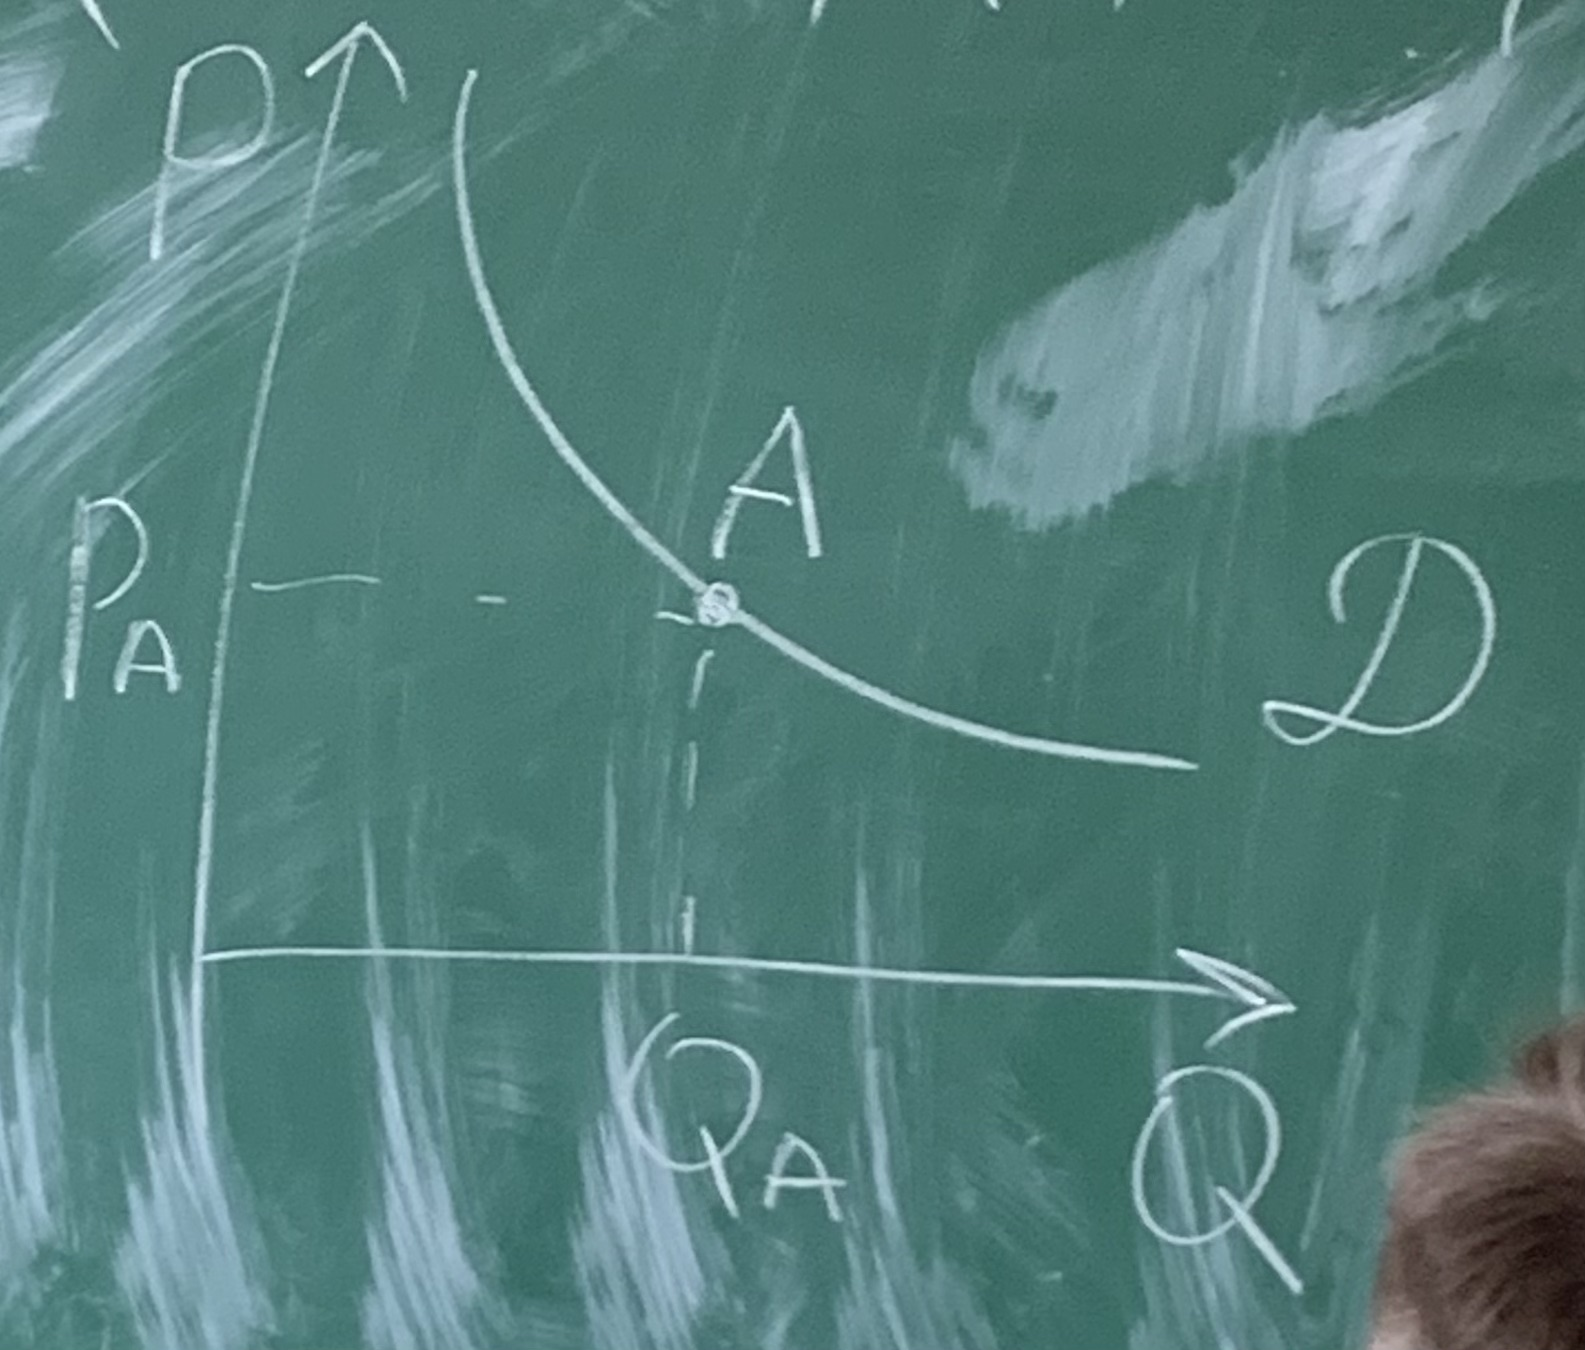
\includegraphics[scale=0.1]{img/spros.JPG}
\end{figure}

Точка $A$ показывает по цене $P_A$ покупатели могут и хотят купить $Q_A$ товара
Функция спроса показывает обратную зависимость между ценой товара и количеством товара, которое покупатель хочет и может купить.

Если меняются не ценовые параметры, то двигается сама кривая.

\subsection{Закон спроса}

При прочих равных условиях как правило чем выше цена товара, тем меньше величина спроса на этот товар и наоборот.

\subsubsection{Парадокс Гиффена}

Малообеспечанные слои населения при повышении цен на предметы первой необходимости увеличивают потребление этих удорожающих товаров. (товары Гиффена). Причина -- вынужненный отказ малообеспеченных слоев населения от потребления других ценных товаров.

\subsubsection{Эффект Веблена}

Высокообеспеченные слои население при повышении цен на товары роскоши увеличивают потребление этих товаров. Причина -- демонстративное потребление

\subsection{Предложение}

Предложение -- это готовность производителя предоставить определенное количество товара за определенный срок при определенных условиях.

\begin{equation}
    Q_S = f(P; P_i; N; T; K; O ...)
\end{equation}

$P$ -- цена на товар $Q$;
$P_i$ -- цены на ресурсы, с помощью которых производят товар $Q$, цены на дополняющие или взаимозаменяющие товары;
$N$ -- налоги;
$T$ -- технологии;
$K$ -- количество товаров на рынке;
$O$ -- ожидание покупателей

\begin{figure}[H]
    \centering
    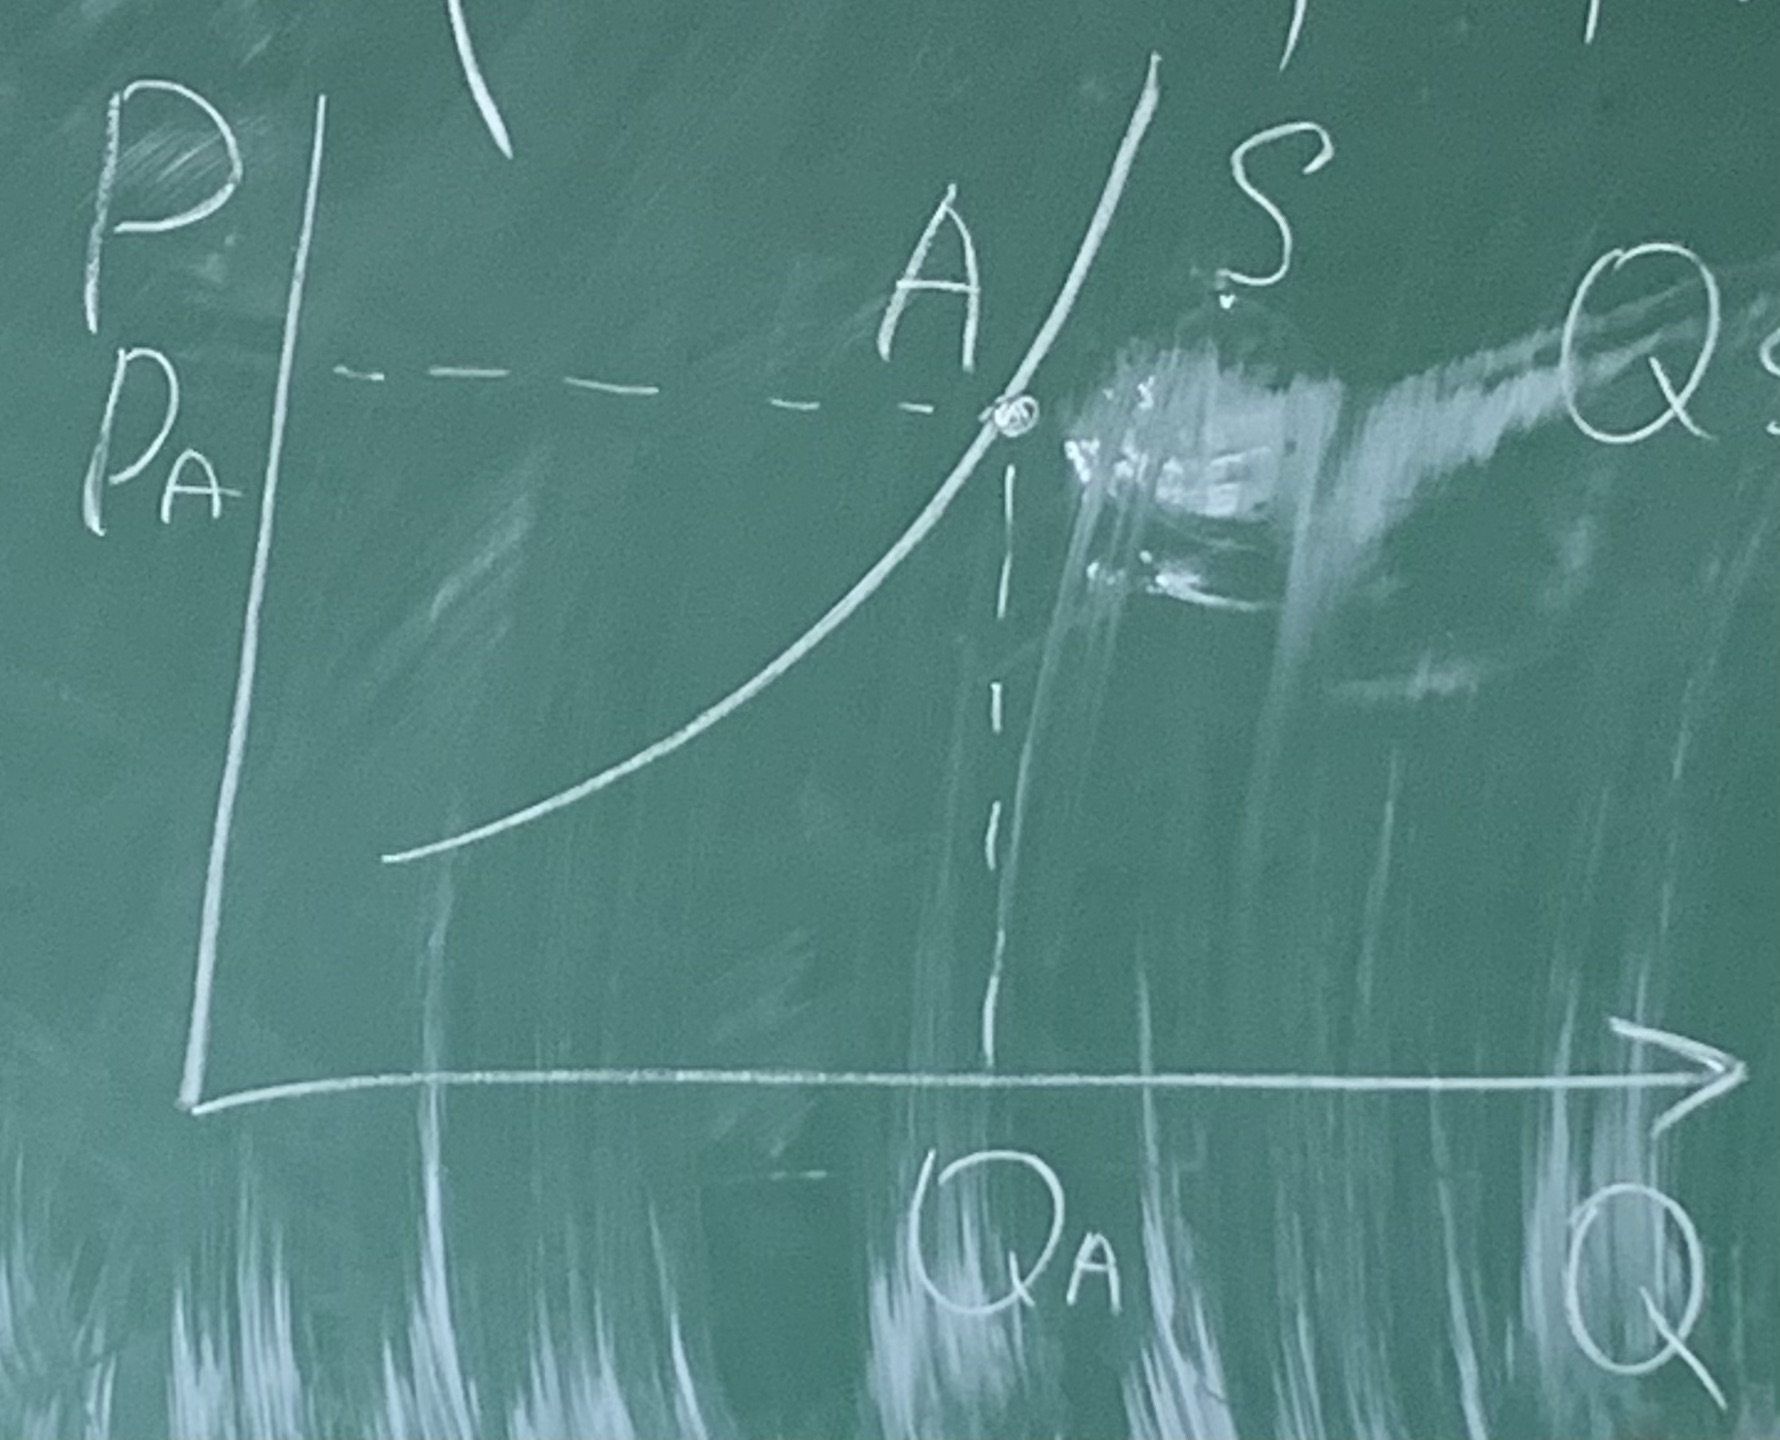
\includegraphics[scale=0.1]{img/predloj.JPG}
    \caption{Функция предложения от спроса}
\end{figure}

Точка $A$ говорит, что продавцы за цену $P_A$ готовы предоставить $Q_A$ товара.

Если меняются не ценовые параметры, то двигается сама кривая.

\subsubsection{Закон предложения}

При прочих равных условиях как правило чем выше цена данного товара, там больше величина предложения данного товара.

\subsection{График спроса и предложения}

\begin{figure}[H]
    \centering
    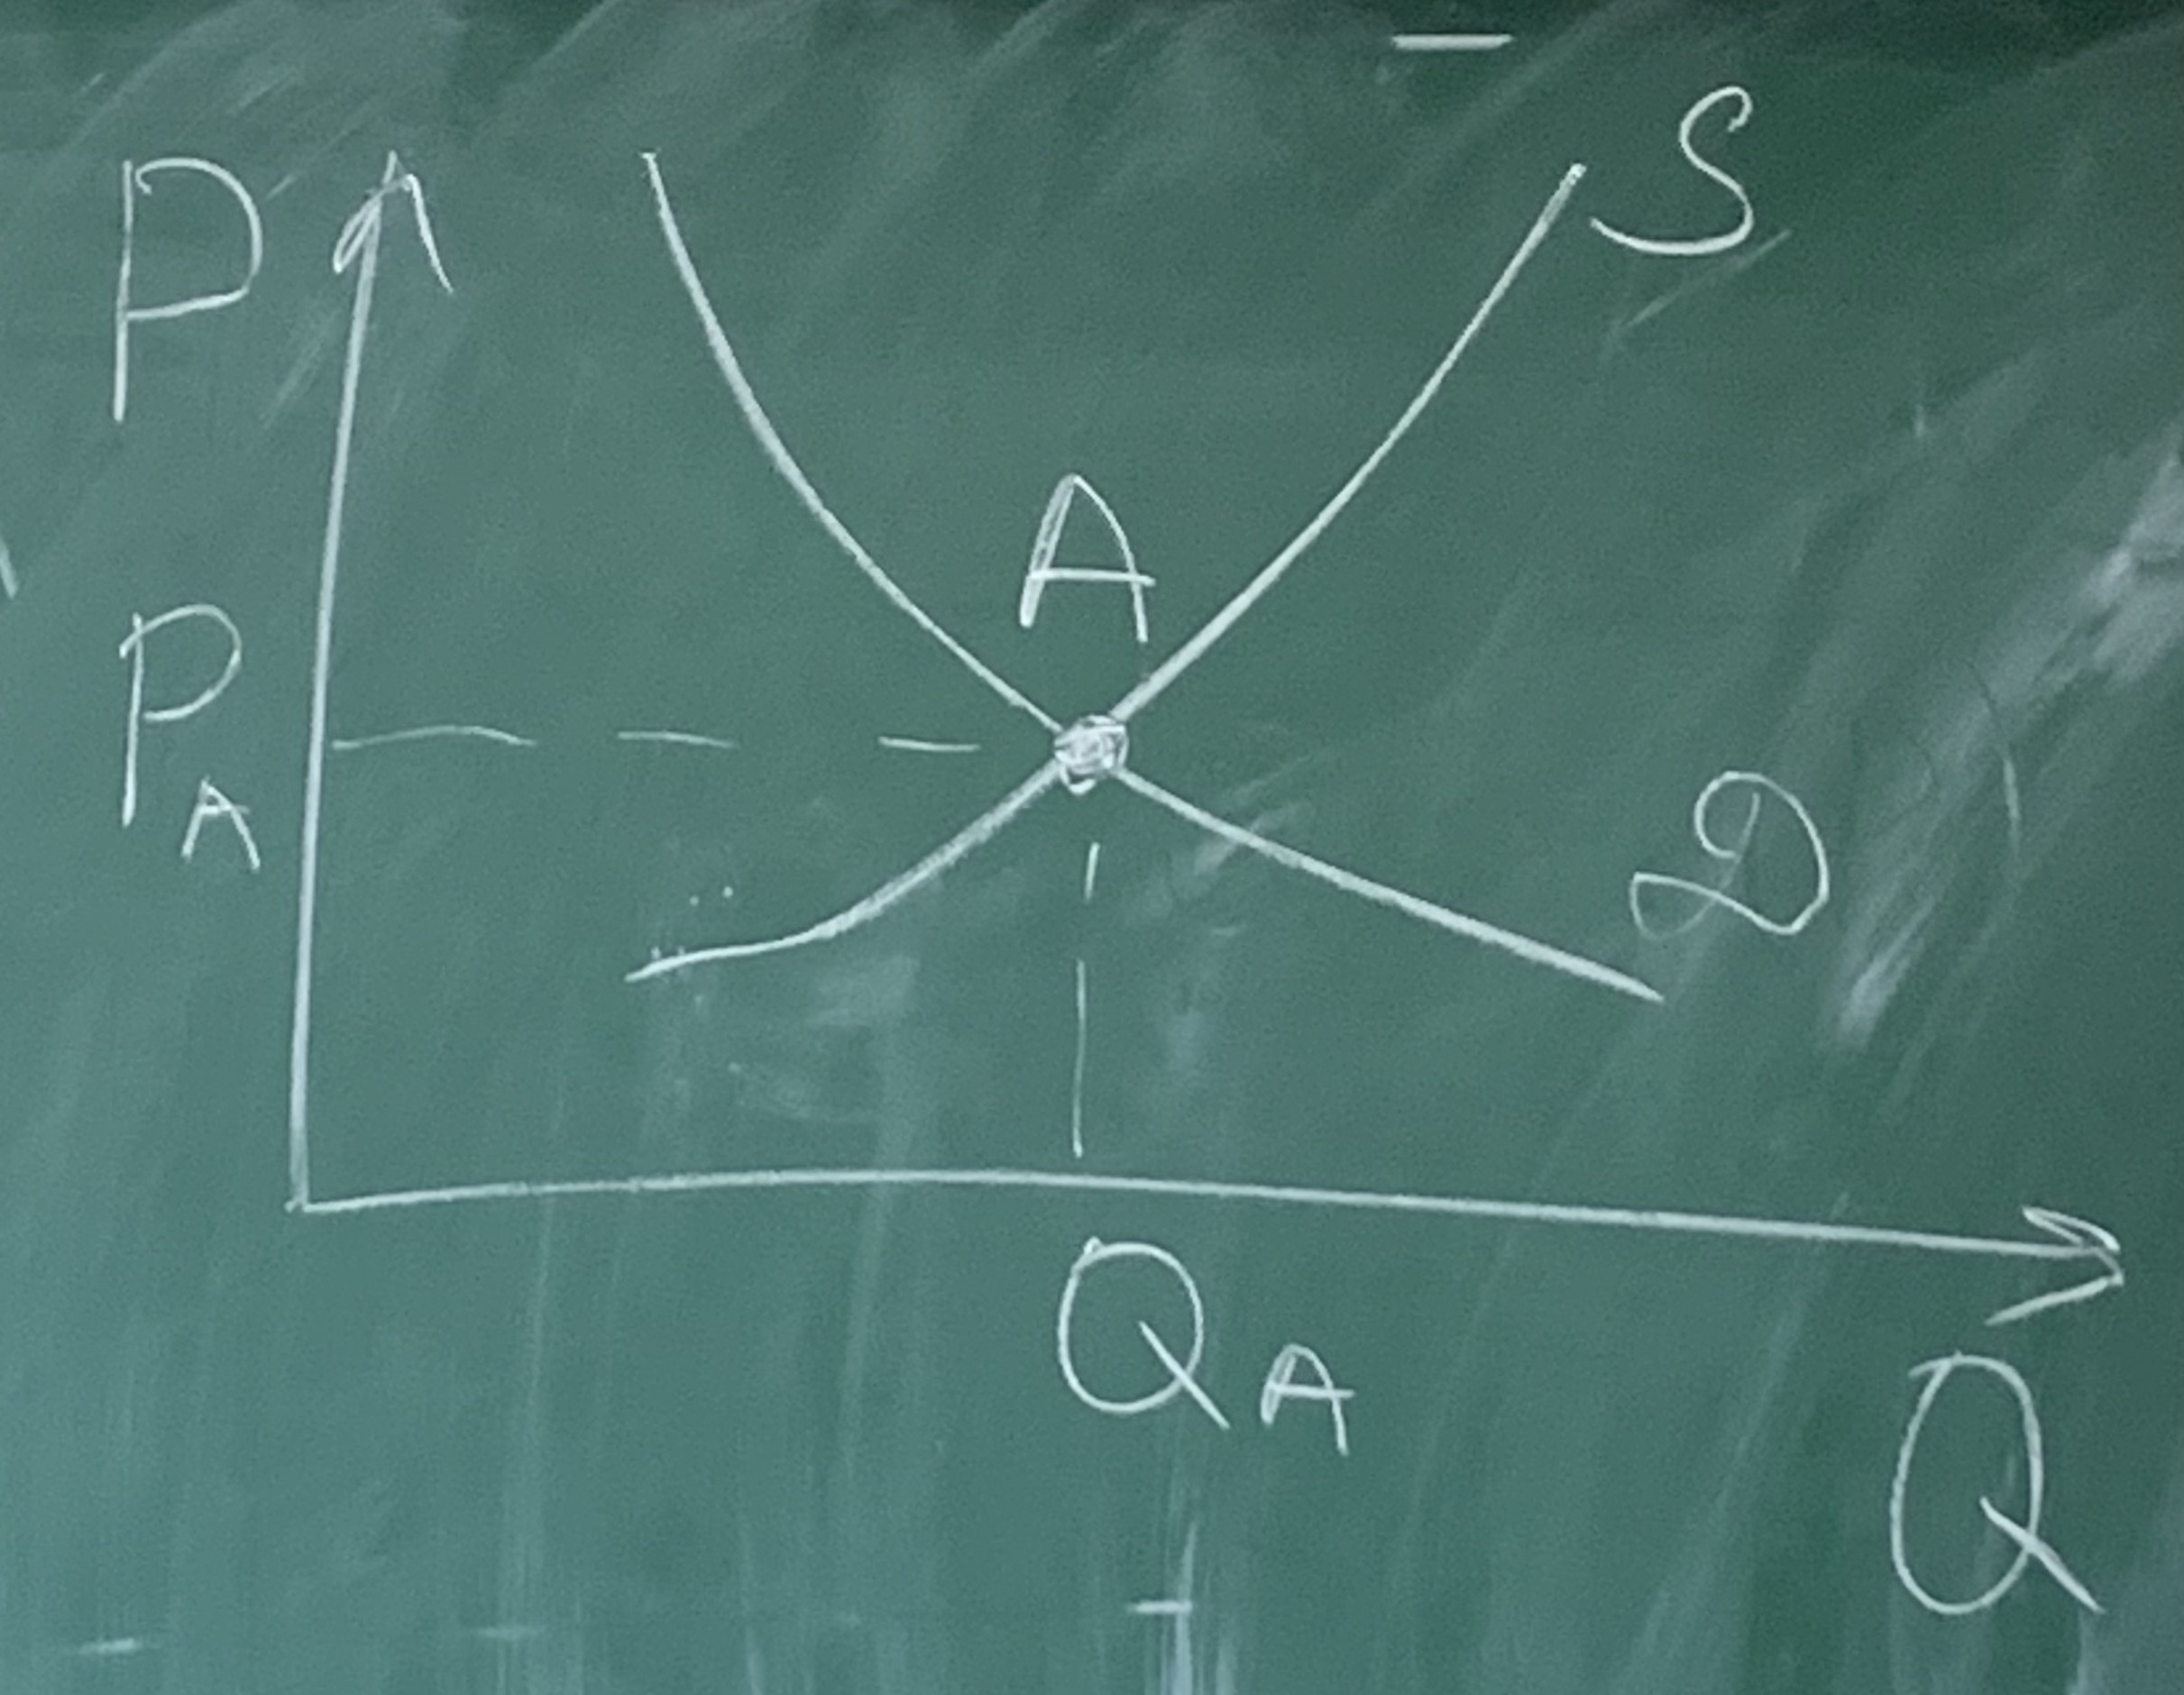
\includegraphics[scale=0.1]{img/krest.JPG}
    \caption{Крест Маршала}
\end{figure}

Если функцию спросаи предложения показать на одном графике, то точка, где функции пересекутся будет точкой равновесия.

\subsection{Задачи}

\subsubsection{Задача 1}

\begin{equation*}
    Q_D = 15 - p
\end{equation*}

\begin{equation*}
    Q_S = -9+3p
\end{equation*}

\begin{equation*}
    Q_S = Q_D \Rightarrow 15 - p = -9 + 3p \Rightarrow p = 6
\end{equation*}

Что произойдет, если объем спроса уменьшится на единицу при любом уровне цен, то функция $Q_D = 15 - p - 1$

\subsection{Задача 3}

Цены на видеомагнитофоны снизилась, что будет на рынке видеокасет?

\subsection{Задача 4}

Дана кривая спроса $D$ на товар $x$. Показать изменения спроса, если товар станет модным.

Переходим в 523

\subsection{Задача 5}

Государство ввело налог на товар $X$, покажите, какие изменения произойдут в предложениях товара.

\subsection{Задача 6}

Изобразите кривую спроса на товар $X$, покажите изменения спроса, если на рынок пришли новые покупатели.

\subsection{Задача 7}

\begin{equation*}
    Q_D = 16 - 4p
\end{equation*}

\begin{equation*}
    Q_S = -2 + 2p
\end{equation*}

\begin{equation*}
    16 - 4p = -2 + 2p \Rightarrow p = 3 \Rightarrow Q_A = 4
\end{equation*}

Объем предложения увеличится на 2 при любом уровне цен

\begin{equation*}
    Q_S = 2p
\end{equation*}

\begin{equation*}
    p = \frac{16}{6} = 2.66
\end{equation*}

\subsection{Задача 8}

Повысились цены на кожу. На производстве обуви соткратили штат. Правильное ли это решение?
